\section{Performance Evaluation}
\label{sec:results}

In this section, we evaluate the performance of our proposed Energy Saving solution in our software-defined O-RAN network. 
Our setup is lightweight, focusing primarily on evaluating the effectiveness of our proposed algorithm rather than the performance of the underlying simulations.
We first discuss the simulation setup, followed by the threshold selection process of various decision variables. 
Our experiments to prove the effectiveness of the proposed algorithm are then presented, followed by a discussion on maintaining QoS guarantees.
In the ensuing graphs, to illustrate the long-term impact of the energy-saving algorithm, we've adopted a time conversion convention where 10 seconds equate to 15 minutes. 

\subsection{Simulation Setup}
Our solution is deployed as an independent rApp, interfacing with the Non-RT RIC and the A1 interface of the O-RAN stack. 
This rApp dispatches decision-making policies to the Near-RT RIC, which houses the TS xApp responsible for reallocating UEs during cell shutdown or bringup processes.
The network, simulated as a Digital Twin using an NS-3 Simulator, comprises eight cells with 20 User Equipments (UEs) per cell, operating in a single-threaded mode.
The rApp operates in a feedback loop with the Digital Twin, obtaining power readings, throughput, and other characteristics across the coverage area.
\textcolor{red}{The network is configured to operate in a 5G New Radio (NR) based CBRS network deployment.}

The Digital Twin in use here is a different one as the one mentioned earlier in the paper in the Algo section \textcolor{blue}{[CITE]}.
The Digital Twin integrated into the ES rApp, is a streamlined simulator that reports selected characteristics of the deployed system, implemented using CloudRF.
The NS-3 simulator serves as the backbone for our network simulation, encompassing the core network, the gNBs, and the UEs. 
The Digital Twin, as previously described, supplements this setup by furnishing the rApp with requisite data.
A more comprehensive explanation of the Digital Twin setup can be provided in the Appendix. [\textcolor{blue}{CITE}]

\subsection{Power Consumption Reduction}

As described in \textcolor{blue}{[CITE]}, the proposed algorithm ensures that the QoS guarantees are maintained during the cell shutdown and bringup processes.
We try to ensure the policy proposed does not lead to a significant drop in the overall CQI of the channels in use for transmission.
We have conducted a series of experiments to evaluate the performance of our proposed solution especially considering the reduction in the power consumption over the given .
First, we look at the performance figures on how the forecasts of the overall throughput help achieve cell shutdown and bringup.

\textcolor{red}{[YOGESH] \\
What is the experiment we are performing? --> A simulation over a certain time-frame, which shows:\\
- Throughput increase or decrease leads to cell shutdown or bringup.\\
- How the power consumption of the system decreases over time.\\
- How the CQI/UE distribution is maintained for atleast a given timeframe \\.
I would like if the first two can be be compared vertically, with time stamps for cell shutdown/bringup maintained. 
The second graph can simply be a comparision of the CQI distribution at the start and the end of the experiment.}

\subsection{Maintaining QoS Guarantees}
\textcolor{red}{[YOGESH] \\
We can view the results in Fig 3. for Cell Shutdown and Bringup both.
Fig 4. shows how our given solution leads to an eventual decrease in total power consumption of the system.
Fig 5. (right now Fig. 2) shows how the CQI distribution is maintained over the given time-frame.}

\begin{figure}[ht]
  \centering
  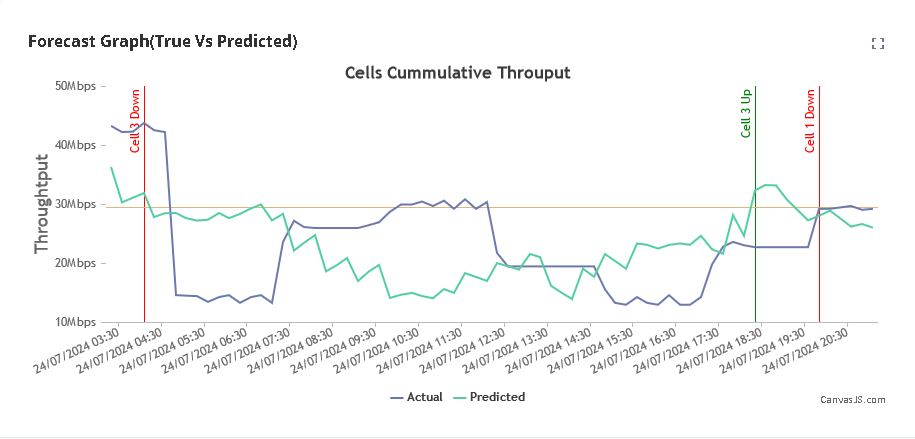
\includegraphics[width=0.4\textwidth]{/Users/pulakmehrotra/Desktop/SaankhyaLabs/es_oran_paper/acm_version_final/images/tpt.png}
  \caption{Throughput Forecasts and Decision Making}
  \label{fig:tpt}
  \end{figure}

\begin{figure}[ht]
  \centering
  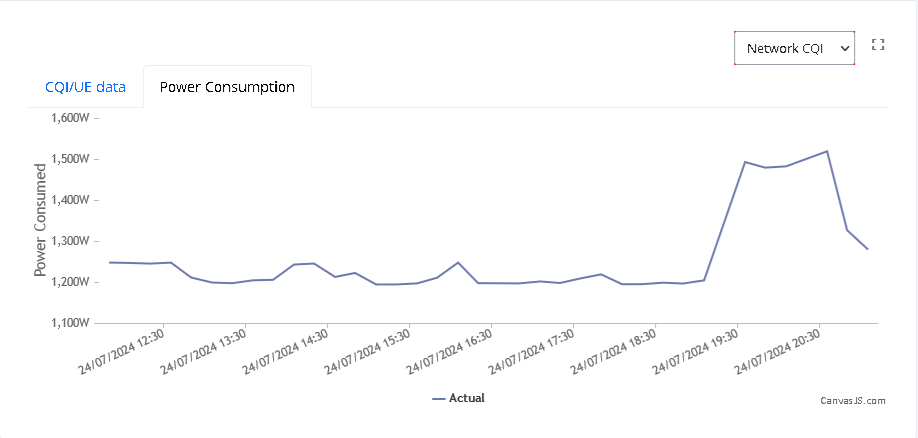
\includegraphics[width=0.4\textwidth]{/Users/pulakmehrotra/Desktop/SaankhyaLabs/es_oran_paper/acm_version_final/images/power_consumption.png}
  \caption{Example of Energy Saving Results}
  \label{fig:power}
  \end{figure}


